\documentclass[letterpaper, 12pt]{article}
\usepackage[a4paper, total={6in, 10in}]{geometry}
\usepackage{svg}
\usepackage{tikz}
\usepackage{float}
\usepackage{lipsum}
\usepackage{wrapfig}
\usepackage{environ}
\usepackage{algorithm}
\usepackage{algpseudocode}
\usepackage{graphicx}
\usepackage{hyperref}
\usepackage{tabularx}
\usepackage{nicematrix}
\usepackage{booktabs}
\svgpath{ {./images/} }
\graphicspath{ {./images/} }
\floatstyle{boxed}

\title{
  
\includegraphics[width=2cm]{unipi_logo.png}\\[1cm]
  Applications of The NEAT Algorithm in Deterministic Game Environments
}
\date{\today}
\author{John Kechagias\\ Department of Informatics, University Of Piraeus}

\makeatletter
\newsavebox{\measure@tikzpicture}
\NewEnviron{scaletikzpicturetowidth}[1]{%
  \def\tikz@width{#1}%
  \def\tikzscale{1}\begin{lrbox}{\measure@tikzpicture}%
  \BODY
  \end{lrbox}%
  \pgfmathparse{#1/\wd\measure@tikzpicture}%
  \edef\tikzscale{\pgfmathresult}%
  \BODY
}
\makeatother
\begin{document}

\maketitle

\begin{abstract}
This paper explores the usages of the NEAT algorithm in combination with self-play in
deterministic game environments. The objective is to investigate the speed at which
models can be trained to adopt particular strategies with minimal reliance on training
data and expert knowledge. To achieve this, we develop a game akin to checkers and use
it as a platform to train models to follow specific strategies.

\parskip=0.5cm

\noindent\textbf{Keywords:} Artificial Neural Networks, NEAT algorithm, Deterministic
Game Environments, Self-play
\end{abstract}

\section*{Introduction}
We aim to address two main shortcomings of RL: data availability, as acquiring sufficient
training date can be prohibitive due to the large state and action space, and lowering the
exploration cost due to the partial observability, sparse feedback and safety concerns that
may incur in real world environments.

The training of models for deterministic game environments goes back a long way

Neuroevolution of augmenting topologies (NEAT) \cite{stanley:ec02} is an evolutionary
algorithm designed for generating artificial neural networks. Developed by Kenneth O.
Stanley and Risto Miikkulainen in 2002, NEAT aims to improve upon traditional
neuroevolution methods by starting with a minimal network topology and gradually
evolving it alongside the connection weights with the goal of keeping the dimentionality
of the search space of connection weights minimal.

This article aims to demonstrate the efficiency of using the NEAT algorithm alongside
self-play to train agents for deterministic game environments.

\section*{Background}
\subsection*{Neuroevolution}
Neuroevolution (NE) is a branch of artificial intelligence that utilizes evolutionary
algorithms to produce artificial neural networks, rules and parameters \cite{neuro19}.
It is primarily applied to general game playing (GGP), robot control and artificial life
\cite{neurogames}. Drawing inspiration from Darwinism, evolutionary algorithms work by
creating successive generations of neural networks mutating them and then evaluating
them. After the networks have been assessed, the fittest of them are selected for
reproduction and create the next generation, leading to fitter offspring in the
long-run. The main advantage of Neuroevolution is that it only requires a measure of a
network's performance at a task, as it searches for a behaviour instead of a value
function. This has two distinct benefits. Firstly, because neuroevolution doesn't take
into account the fitness landscape, as opposed to more generally used optimization
methods like gradient descent, it is less likely to get stuck on local minima. Secondly,
it doesn't require curated datasets of input-output pairs, as opposed to supervised
learning algorithms.

In traditional NE approaches, evolving networks have a predetermined structure that is
chosen before the experiment. This usually corresponds to a single hidden layer where
each neuron is connected to all input and output neurons. By using a fixed layout of
neurons the problem becomes a weight optimization problem where we search through the
weight space for optimal values. However, it isn't always easy to select a good
representation in advance. Firstly, the complexity of the structure should reflect the
complexity of the problem, therefore a singular structure cannot be ideal for all
problems. Secondly, although a single hidden layer is able to represent any function, it
does not mean that every function can be easily represent by one. This can be partially
solved by the addition of subsequent hidden layers, but this grows and complexifies the
search space exponentially. Additionally, the growth of the search space exacerbates the
problem of competing conventions, where different networks correspond to the same
function and crossover leads to damaged offspring. This paradigm of static
representations shifted in the 1990s with the emergence of topology and weight evolving
artificial neural networks (TWEANNs). These new methods introduced new mutations to the
evolutionary process that altered the structure of the networks; for instance, the
addition of a neuron or connection.

\subsection*{Competing Conventions Problem}
The problem of competing conventions \cite{schafwhit}, also known as the Permutations
Problem \cite{Radcliffe1993GeneticSR} arises in evolutionary algorithms when different
networks correspond to the same function. During crossover, these networks are likely to
yield offspring that deviate significantly from the original function, leading to a loss
in innovation.

\subsection*{Neuroevolution of Augmenting Topologies}
One of the most successful TWEANN algorithms is NEAT (Neuroevolution of augmenting
topologies) \cite{stanley:ec02}. Developed by Kenneth O. Stanley and Risto Miikkulainen
in 2002, NEAT borrows a lot of concepts from genetic algorithms \cite{lamangup} and aims
to improve upon its TWEANN predecessors. It provides meaningful crossover of different
topologies through the tracking of the historical origin of genes, protects
underdeveloped innovations through speciation and keeps topologies small by starting
with a minimal structure and incrementally growing it. 

NEAT has proven to be an efficient solution for reinforcement problems where the cost
function is not easily defined. Networks are also able to avoid local optima and develop
a wide range of strategies as NEAT tries to preserve innovations by speciating the
models based on their similarity. Networks are given time to optimize their new
structural innovations instead of being discarded due to their short-term dip in
fitness. This leads to species developing distinct strategies. Moreover, since NEAT only
requires a measure of a networks performance to function it can be used for training
models on games without relying on expert knowledge.

NEAT uses a variable-length genetic encoding where each individual (Genome) has a list
of node genes and a list of connection genes:
\begin{itemize}
  \item Node genes represent network nodes. They hold information such as the node type
    (input, output, hidden) as well as its innovation number. 
  \item Connection genes represent the connection between two nodes. They hold
    information such as the input node, output node, connection weight, an enable bit
    (whether or not the gene is expressed) and an innovation number.
\end{itemize}

There are four kinds of generic mutations: two structural mutations, a weight mutation
and a mutation that alters the enable bit. The structural mutations  expand the network
by either adding a node between an existing connection or a connection between existing
nodes (see Figures \ref{fig:add_node}, \ref{fig:add_con}). In addition, there is the
common weight mutation present in multiple other such methods where the weight of
connections is either set to a random value, set to a default value or slightly altered
based on a distribution. Finally, there is the mutation that alters the enable bit,
thereby altering the expression of the gene.

\begin{figure}[H]
  \centering
  \includesvg[width=0.9\textwidth]{add_node.svg}
  \caption{Add node mutation.}
  \label{fig:add_node}
  \vspace{1cm}
  \includesvg[width=0.9\textwidth]{add_connection.svg}
  \caption{Add connection mutation.}
  \label{fig:add_con}
\end{figure}

\subsubsection*{Tracking of Genes}
One problem that every genetic algorithm has to solve is the problem of competing
conventions. NEAT solves this by using innovation numbers that acts as identifiers for
structural innovations. An innovation number is an extra property that is attached to
genes and works like an ID. When a structural mutation occurs, it is paired with an
innovation number and saved on an innovation record table. The same innovation number is
used as the ID of the produced gene. New, higher numbers are generated for each
additional gene. Whenever a structural mutation occurs we first check if it has already
been registered on the innovation record table, if it has we make sure to use the same
identifiers as previously. This allows for the same structural mutation to be identified
as the same across all genomes and generations.

\begin{figure}[H]
    \centering
    \includesvg[width=0.9\textwidth]{innovation_record.svg}
    \caption{
      Structural mutation in NEAT. A node with ID 5 is added between nodes 2 and 4. This
      addition is recorded by adding a new entry in the innovation record, linking the
      mutation of the connection (2,4) with the innovation number 5. Subsequently, if
      the connection (2,4) is mutated in any network the produced node will be assigned
      ID 5. This can also be interpreted as node 5's ancestor being the connection
      (2,4).
    }
\end{figure}

The utilization of innovation numbers not only addresses the problem of competing
conventions, but it also simplifies crossover, as it removes the need for expensive
topological analysis. Crossing over two genomes is done by lining up their innovation
number in chronological order (ascending order). Matching genes are inherited randomly,
whereas nonmatching genes are are inherited from the more fit parent.

\subsubsection*{Speciation}
To maximize the solution space covered, a diverse population of varying topologies is
required. Since different topologies evolve at different rates, a mechanism is required
to safeguard them from unfair competition. NEAT addresses this by introducing
speciation. In each generation, genomes are separated into species based on a distance
metric, allowing them to compete primarily within their own niche. The bigger the
distance the more dissimilar the genomes are. The distance is computed by taking into
account the number of genes in the largest genome \(N\), excess \(E\) and disjoint \(D\)
genes, as well as the overage weight differences of matching genes \(\overline{W}\),
including disabled genes:

\[\delta=\frac{c_1E}{N}+\frac{c_2D}{N}+c_3 \cdot \overline{W}\]

The hyperparameters \(c_1\), \(c_2\) and \(c_3\) help fine-tune the function. Genomes
whose distance fails below a given threshold can be grouped into the same species.
Subsequently, genomes are assigned to the most similar species. If a genome does fails
to be assigned to a preexisting species it creates a new one. In addition, an explicit
fitness sharing \cite{goldbergarichardson} is employed to make it hard for any species
to grow large enough to take over the entire population. The method works by allotting
each species a number of offspring slots that is proportional to the average fitness of
its members. Within each species, individuals then compete with other for the change to
reproduce. A select number of the fittest individuals reproduce via crossover, while all
the other individuals are discarded. Each population replaced in its entirety by its
offspring.

\subsubsection*{Growing From Minimal Topology}
Many predecessors of NEAT had their initial population be random topologies. While this
approach ensures topological diversity from the start, it also introduces optimization
problems, as random topologies are bound to have unnecessary genes that need time to be
filtered out. NEAT adopts a different strategy. By starting with a population of
topologies that only include the input and output nodes it eliminates the extra time
required to weed out unnecessary genes and ensures that only necessary genes are
included.

\subsection*{Self-Play}
Self-play, a technique where agents learn by competing against variations or copies of
themselves, has emerged as a powerful tool in multi-agent reinforcement learning (MARL)
\cite{5392560}. In this approach, agents train by interacting with copies of themselves,
enabling a gradual escalation of challenge and complexity within the learning
environment. Notably, one major advantage of this technique is its nonnecessity for
training data, thereby eliminating the need for pre-collected datasets. A seminal
contribution to this field is AlphaGo Zero \cite{silver2017mastering}, a model trained
to play the board game Go, which achieved remarkable results against human players by
utilizing a self-play learning schema. In our study, we use an approach similar to that
of AlphaGo Zero. Self-play is employed to enhance our fitness function.

\section*{Methodology}
To evaluate NEAT in a deterministic game environment we created a game similar to
checkers with incorporated elements from the board game \textbf{Catan}. The idea is to
use the NEAT algorithm in conjunction with self-play to train neural models based on
specific game strategies. We monitor and evaluate their progress and lastly, do a live
assessment where the best model faces off against a human opponent. To accomplish this
three components are required: the custom game itself, an algorithm employing a neural
model for gameplay and a system for training the neural models using NEAT and self-play.

For our purposes, a system was developed utilizing the NEAT algorithm and self-play that
allows for the relatively quick training and evaluation of agents. It allows users to
define their own fitness function and adjust the process through parameterization. To
address the need for parallel training and evaluation of multiple agents, we have
utilized Python's built-in multiprocessing module and Numba, a just-in-time (JIT) Python
compiler.

\section*{Game Rules}
The game is played on a five by five board with hexadecimal tiles (see Figures
\ref{fig:transfer_move}, \ref{fig:production_move}). There are two players, denoted as
\textbf{red} and \textbf{blue}. Players start on opposite corners of the board with one
piece each. Each board tile can hold a maximum of ten pieces. We say that a player owns
a tile when he has pieces on it. The blue player moves first and then play alternates
between sides. The goal of the game is to eliminate all of the opponent's pieces. There
are two moves available to each player, \textbf{transfer} and \textbf{production}.

\subsection*{Transfer Move}
Players can select any number of their owned pieces from a tile and transfer them to a 
neighbouring tile. For this move to be valid, the following conditions must be met:
\begin{itemize}
  \item The starting tile and the destination tile are adjacent.
  \item The number of selected pieces must not exceed the total number of pieces on the
    starting tile.
  \item The total number of pieces on the destination tile must not exceed the maximum 
    allowed number of pieces on a tile.
\end{itemize}
If the destination tile is occupied by the opposing player, a fight ensues. During the
fight, the number of tiles possessed by the player with the greater quantity is
subtracted from both sides. For example, blue player transfers six troops from tile
\((4, 0)\) to \((3, 1)\):


\begin{figure}[H]
  \begin{minipage}[c]{.5\textwidth}
    \centering
    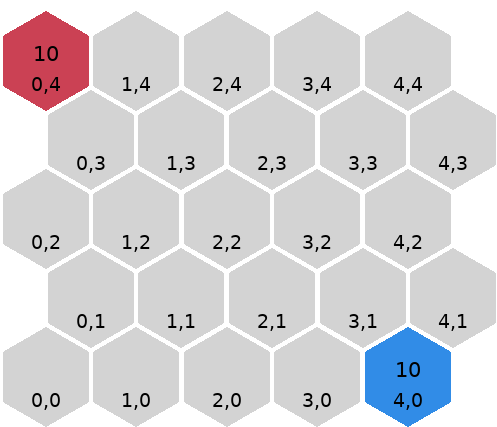
\includegraphics[width=0.9\textwidth]{transfer_example_1.png}
    \caption{Before the Transfer Move.}
    \label{fig:transfer_move}
  \end{minipage}%
  \begin{minipage}[c]{.5\textwidth} \centering
    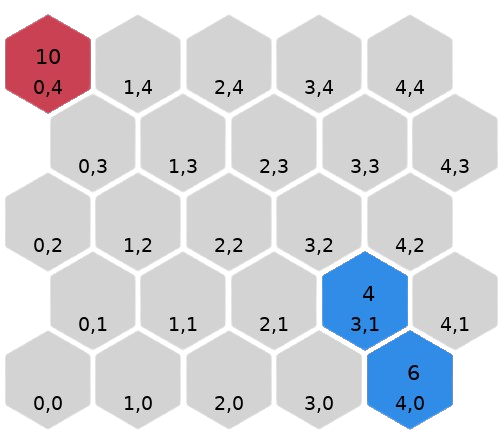
\includegraphics[width=0.9\textwidth]{transfer_example_2.png}
    \caption{After the Transfer Move.}
  \end{minipage}
\end{figure}

\subsection*{Production Move}
Players can select a tile they occupy and add one more piece to it. For this move to be
valid, the number of pieces on the tile must be less than the maximum allowed number of
pieces on a tile. For example, blue player produces a piece on tile \((3, 1)\):

\begin{figure}[H]
  \begin{minipage}[c]{.5\textwidth}
    \centering
    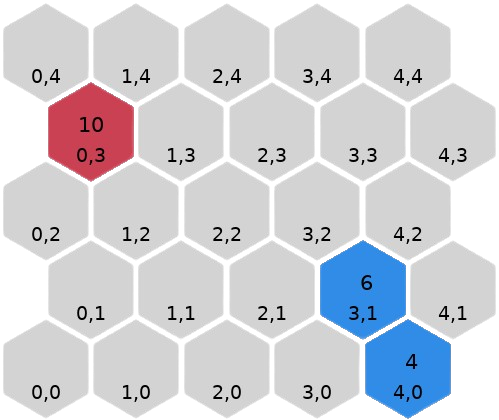
\includegraphics[width=0.9\textwidth]{production_example_1.png}
    \caption{Before the Production Move.}
    \label{fig:production_move}
  \end{minipage}%
  \begin{minipage}[c]{.5\textwidth} \centering
    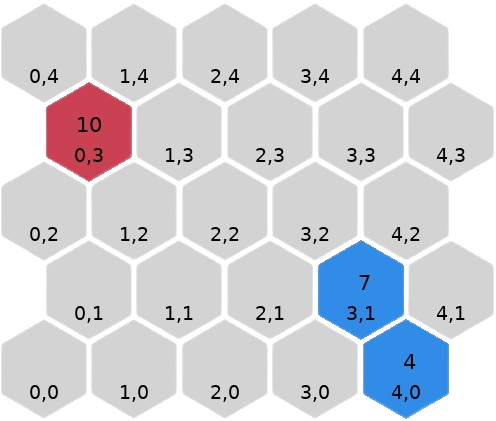
\includegraphics[width=0.9\textwidth]{production_example_2.png}
    \caption{After the Production Move.}
  \end{minipage}
\end{figure}

\section*{Gameplay Algorithm}
The gameplay algorithm works as follows. The idea is to search through the available
move tree of a player up to a specified depth and use a neural network to evaluate each
corresponding game state. The neural network takes the matrix representation of the game
state and outputs a score that represents how advantageous the position is for the
moving player. Then, the algorithm chooses and plays the move which results in the most
advantageous position. To search through the move tree we use the principal variation
search (PVS) algorithm, an enhanced version of alpha-beta pruning \cite{Brud1963}.

\subsection*{Principal Variation Search}
Before explaining how the principal variation algorithm works we have to explain the
concept of the principal variation. The principal variation is the sequence of moves
that players determine to be the best possible outcome given their analysis of the
current position. In other words, it is the line of play that both sides believe will
lead to the most advantageous position for them.

The Principal Variation Search algorithm (PVS) \cite{Mar1982} represents an enhancement
of the alpha-beta algorithm. It relies on effective move sorting, as it is structured
around the concept that moves positioned closer to the beginning of the move list are
generally better and more likely to be part of the principal variation. This
prioritization allows the PVS algorithm to save time by primarily exploring moves deemed
to be within the principal variation. By initially probing the most promising paths, PVS
can effectively prune the search tree, discarding less relevant branches
\cite{Mar1985}. Moreover, it operates under the 'fail-soft' principle,
meaning that if an earlier move in the sorted list fails high (produces a cutoff with a
value greater than or equal to beta), subsequent moves are searched with a reduced
window around the previous result. This approach not only accelerates the search process
but also enables the algorithm to focus its efforts on the most promising paths, leading
to more accurate evaluations. To further improve the performance of the algorithm,
multiple optimization techniques have been applied like singular extensions, late move
reduction and the utilization of a transposition table.

\begin{scaletikzpicturetowidth}{\textwidth}
\begin{tikzpicture}[scale=\tikzscale,font=\footnotesize]
\tikzstyle{solid node}=[circle,draw,inner sep=1.5,fill=black]
\tikzstyle{hollow node}=[circle,draw,inner sep=1.5]
\tikzstyle{level 1}=[level distance=15mm,sibling distance=3.5cm]
\tikzstyle{level 2}=[level distance=15mm,sibling distance=1.5cm]
\tikzstyle{level 3}=[level distance=15mm,sibling distance=1cm]
\node(0)[solid node,label=above:{$P1$}]{}
child{node[solid node,label=above left:{$P2$}]{}
child{node[hollow node,label=below:{$(1,2)$}]{} edge from parent node[left]{$C$}}
child{node[hollow node,label=below:{$(1,-1)$}]{} edge from parent node[left]{$D$}}
child{node[hollow node,label=below:{$(0,2)$}]{} edge from parent node[right]{$E$}}
edge from parent node[left,xshift=-5]{$A$}
}
child{node[solid node,label=above right:{$P2$}]{}
child{node[hollow node,label=below:{$(2,2)$}]{} edge from parent node[left]{$F$}}
child{node[hollow node,label=below:{$(1,3)$}]{} edge from parent node[right]{$G$}}
edge from parent node[right,xshift=5]{$B$}
};
\end{tikzpicture}
\end{scaletikzpicturetowidth}

\section*{Model Training}

\subsection*{NEAT Implementation Overview}
In addition to the system for the training of agents, we also developed a Python
implementation of the NEAT algorithm.
\footnote{\url{https://github.com/JohnKechagias/neat-proc}}. The implementation is based
on the original paper \cite{stanley:ec02}. The core algorithm remained unchanged with
some additions, elite genomes and interspecies crossover. For our purposes, we opted for
feedforward neural networks. As a result, all standard mutations have been redesigned to
ensure the networks maintain their feedforward structure. The following steps are done
in every iteration of the evolutionary process:
\begin{enumerate}
  \item Speciation.
  \item Evaluation of genomes.
  \item Filtering of stagnant species.
  \item Crossover and mutation.
\end{enumerate}

\subsubsection*{Genes}
The gene design follows NEAT's default approach with some adjustments. Node genes store
information related to the innovation number, node type, bias, response, aggregation
function, and activation function. On the other hand, connection genes store information
regarding the innovation number, input node, output node, weight, enabled status, and
frozen status. If a connection is frozen, its weight is not subject to mutations. The
node and connection parameters are shown in Tables \ref{table:node_params} and
\ref{table:connection_params} respectively.

\subsubsection*{Genomes}
The genome used is a direct encoding scheme made by a list of connections genes and a
list of node genes. The genome parameters are shown in Table \ref{table:neat}.

\subsubsection*{Species Elites}
In the original NEAT implementation, every reproduction cycle involves replacing the
entire population with offspring. This approach risks discarding innovations developed
by the more fit individuals, since there is no guarantee that their offspring will
inherit them. To avoid this, a new mechanism named \textbf{species elites} is
introduced. The elites of each species are its fittest members, with the maximum number
of elites for each species being specified by a hyperparameter. During the reproduction
phase, the elites of each species are copied over to the new population. Consequently,
the new population consists not only of offspring, but also the elites of each species.
To prevent the inclusion of elites from underdeveloped species, namely those with a
small population, a hyperparameter is introduced to specify the minimum size required
for a species to have its elites copied over.

\subsubsection*{Interspecies Crossover}
Although speciating the population allows structures to develop at their own pace, it
can also lead to over-specialization. This occurs when a large majority of the fittest
individuals of a species develop overly similar structures over time, leading to overly
similar offspring. This constitutes an innovation drought for the species, jeopardizing
its long-term viability and cannot be easily offset by mutations, as the mutation rate
must be within a specific range for individuals to remain stable enough to retain and
develop useful features. Allowing interspecies crossover can help introduce new features
to species and can also lead to offspring inheriting the best of their parents' worlds.
It is vital that the interspecies crossover rate remains relatively low, as larger
values undermine the speciation mechanism.

\subsection*{Input Preparation}
The following protocol was adopted for evolving strategies in the aforementioned game.
The game board is interpreted as a five by five matrix, with each cell representing a
tile on the board. The value in each cell shows the number of soldiers present on that
tile. In order to differentiate between players' pieces, blue pieces are represented with
positive numbers and red pieces with negative numbers.

\subsection*{Move Searching} 
The idea is to search through all the possible moves and countermoves up to a given
depth and utilize the neural network for assessing each game state. The job of the
neural networks is to take the matrix form of a game state as input and output a score
indicating how favourable the position is for the player whose pieces are represented
with positive numbers. Since the networks are designed to evaluate positions only from
the perspective of the player with positive pieces, when we want to evaluate a position
from the perspective of the other player (whose pieces are represented with negative
numbers), we must multiply the matrix by \(-1\) to switch perspectives. We employ the
principal variation search to examine all possible moves up to a given depth. For
evaluating each game state we utilize the neural network. Whenever we change player
turns, we adjust the matrix by multiplying it by \(-1\) before feeding it to the model
to switch perspectives. Once the search is complete, we select the move that results in
the most advantageous game state for the current player.

\subsection*{Fitness Function}
Given that NEAT is a genetic algorithm variant, the fitness function plays a vital role
for in ensuring its proper function. The fitness value serves as a measure of how adept
an individual is for the task. Self-play was utilized to evaluate the genomes. The
intention is to pit the genomes against the best of the previous generation and
calculate their fitness based on the game results. For the first run, because a previous
generation does not exist, we pick five genomes at random to act as the opponents. Each
genome fights a set amount of times against each opponent in order to get an average
score for each fight. After all games are completed, we take the average of the game
scores and assign it as the fitness of the genome. The function that outputs a score
based on a game record, not only takes into account the game's result, but also the
moves that the model made.

\section*{Appendix}

\begin{table}[H]
\centering
\caption{NEAT Parameters}
\label{table:neat}
\begin{NiceTabular}{X|c}
\toprule
\textbf{Hyperparameters} & \textbf{Values} \\
\midrule
Population  & 200 \\
Input Nodes  & 25 \\
Output Nodes  & 1 \\
Hidden Nodes & 0 \\
Feed-Forward & True \\
Connection Scheme & Fully Connected \\
Fitness Threshold & 400 \\
\bottomrule
\end{NiceTabular}
\end{table}

\begin{table}[H]
\centering
\caption{Node Gene Parameters}
\label{table:node_params}
\begin{NiceTabular}{X|c}
\toprule
\textbf{Hyperparameters} & \textbf{Values} \\
\midrule
Node Mutation Chance & 1.0 \\
Node Addition Chance & 0.2 \\
Node Deletion Chance & 0.2 \\

Activation Function & Sigmoid \\
Activation Function Options & [Sigmoid] \\
Activation Function Mutation Chance & 0.0 \\

Aggregation Function & Summation \\
Aggregation Function Options & [Summation] \\
Aggregation Function Mutation Chance & 0.0 \\

Bias Initial Mean & 1.0 \\
Bias Initial Standard Deviation & 1.0 \\
Bias Minimum Value & -30 \\
Bias Maximum Value & 30 \\
Bias Mutation Chance & 0.7 \\
Bias Reset Chance & 0.1 \\
Bias Mutation Power & 0.5 \\

Response Initial Mean & 1.0 \\
Response Initial Standard Deviation & 0.0 \\
Response Minimum Value & -30 \\
Response Maximum Value & 30 \\
Response Mutation Chance & 0.0 \\
Response Reset Chance & 0.0 \\
Response Mutation Power & 0.0 \\
\bottomrule
\end{NiceTabular}
\end{table}

\begin{table}[H]
\centering
\caption{Connection Gene Parameters}
\label{table:connection_params}
\begin{NiceTabular}{X|c}
\toprule
\textbf{Hyperparameters} & \textbf{Values} \\
\midrule
Connection Mutation Chance & 1.0 \\
Connection Addition Chance & 0.5 \\
Connection Deletion Chance & 0.5 \\
Connection Enable By Default & True \\
Connection Enable Mutation Chance & 0.01 \\
Connection Frozen By Default & False \\
Connection Frozen Mutation Chance & 0.0 \\

Weight Initial Mean & 0.0 \\
Weight Initial Standard Deviation & 1.0 \\
Weight Minimum Value & -30 \\
Weight Maximum Value & 30 \\
Weight Mutation Chance & 0.8 \\
Weight Severe Mutation Chance & 0.01 \\
Weight Reset Chance & 0.1 \\
Weight Mutation Power & 0.5 \\
\bottomrule
\end{NiceTabular}
\end{table}

\begin{table}[H]
\centering
\caption{Speciation Parameters}
\begin{NiceTabular}{X|c}
\toprule
\textbf{Hyperparameters} & \textbf{Values} \\
\midrule
Compatibility Disjoint Coefficient & 1.0 \\
Compatibility Weight Coefficient & 0.5 \\
Species Fitness Function & Maximum \\
Species Elitism & 2 \\
Species Maximum Stagnation & 15 \\
Survival Rate & 0.2 \\
Elitism & 2 \\
\bottomrule
\end{NiceTabular}
\end{table}

\begin{table}[H]
\centering
\caption{Reproduction Parameters}
\begin{NiceTabular}{X|c}
\toprule
\textbf{Hyperparameters} & \textbf{Values} \\
\midrule
Crossover Rate & 1.0 \\
Interspecies Crossover Rate & 0.15 \\
Maximum Stagnation & 20 \\
Survival Rate & 0.2 \\
Elitism & 2 \\
Elitism Threshold & 2 \\
Minimum Species Size & 2 \\
\bottomrule
\end{NiceTabular}
\end{table}

\bibliographystyle{plain}
\bibliography{refs}
\end{document}
